%%%%%%%%%%%%%%%%%%%%%%%%%%%%%%%%%%%%%%%%%%%%%%%%%%%%%%%%%%%%%%%%%%%%%%%%%%%

%
% Plantilla para un artculo en LaTeX en espaol.
%
%%%%%%%%%%%%%%%%%%%%%%%%%%%%%%%%%%%%%%%%%%%%%%%%%%%%%%%%%%%%%%%%%%%%%%%%%%%

\documentclass[a4paper, 11pt, oneside]{article}


% idioma
\usepackage[utf8]{inputenc}
\usepackage[spanish]{babel}
\usepackage{enumerate}
\usepackage{multirow} % para las tablas
\usepackage{soul}
\usepackage{graphicx}

%tablas
\usepackage{booktabs}

%rotar tablas
\usepackage{rotating}

%color tablas
\usepackage{colortbl}

%espaciado
\usepackage{setspace}
\onehalfspacing
\setlength{\parindent}{0pt}
\setlength{\parskip}{2.0ex plus0.5ex minus0.2ex}


%margenes según n. icontec
\usepackage{vmargin}
\setmarginsrb           { 4.0cm}  % left margin
                        { 4.0cm}  % top margcm
                        { 2.0cm}  % right margcm
                        { 3.0cm}  % bottom margcm
                        {  10pt}  % head height
                        {0.25cm}  % head sep
                        {   9pt}  % foot height
                        { 0.3cm}  % foot sep


% inserción url's notas de pie.
\usepackage{url}


% Paquetes de la AMS:
\usepackage{amsmath, amsthm, amsfonts}

% Paquete para resaltar texto con una caja amarilla para correcciones
\usepackage{color}
\newcommand{\hilight}[1]{\colorbox{yellow}{#1}}

% Teoremas
%--------------------------------------------------------------------------
\newtheorem{thm}{Teorema}[section]
\newtheorem{cor}[thm]{Corolario}
\newtheorem{lem}[thm]{Lema}
\newtheorem{prop}[thm]{Proposición}
\theoremstyle{definition}
\newtheorem{defn}[thm]{Definición}
\theoremstyle{remark}
\newtheorem{rem}[thm]{Observación}

% Atajos.
% Se pueden definir comandos nuevos para acortar cosas que se usan
% frecuentemente. Como ejemplo, aqu se definen la R y la Z dobles que
% suelen representar a los conjuntos de nmeros reales y enteros.
%--------------------------------------------------------------------------

\def\RR{\mathbb{R}}
\def\ZZ{\mathbb{Z}}

% De la misma forma se pueden definir comandos con argumentos. Por
% ejemplo, aqu definimos un comando para escribir el valor absoluto
% de algo ms fcilmente.
%--------------------------------------------------------------------------
\newcommand{\abs}[1]{\left\vert#1\right\vert}

% Operadores.
% Los operadores nuevos deben definirse como tales para que aparezcan
% correctamente. Como ejemplo definimos en jacobiano:
%--------------------------------------------------------------------------
\DeclareMathOperator{\Jac}{Jac}



\newcommand\portada{
\begin{titlepage}
		\begin{center}
			{\large \bf Diseño y prueba de una arquitectura computacional segura para compartir información entre el Hospital del Sur, Instituto Nacional de Salud y la Red de Monitoreo de Calidad del Aire de Bogotá.}
            
			\vfill
 			{\large\bf PRESENTADO POR: \par}
			{\large\bf Marco Antonio Méndez \par}
            {\large\bf Hoffman Antonio Márquez}
			\vfill
			{\large\bf UNIVERSIDAD ANTONIO NARIÑO  \par}
			{\large\bf FACULTAD DE INGENIERÍA DE SISTEMAS \par}
			{\large\bf INGENIERIA DE SISTEMAS Y COMPUTACIÓN \par}
			{\large\bf BOGOTÁ D.C.\par}
			{\large\bf MAYO 16 DEL 2016 \par}
		\end{center}
\end{titlepage}
}

\newcommand\contraportada{
	\begin{titlepage}
		\begin{center}
{Diseño y prueba de una arquitectura computacional segura para compartir información entre el Hospital del Sur, Instituto Nacional de Salud y la Red de Monitoreo de Calidad del Aire de Bogotá.} 
			\vfill
 			{\large\bf PRESENTADO POR: \par}
			{\large\bf Marco Antonio Méndez \par}
            {\large\bf Hoffman Antonio Márquez}
			\vfill
			{\large\bf Anteproyecto de grado \par}
			\vfill
			{\large\bf Directores: Ing. David Alberto Herrera Alvarez PhD. / Ing. Raúl Ernesto Menéndez Mora PhD. 
\par}
			\vfill
			{\large\bf UNIVERSIDAD ANTONIO NARIÑO \par}
			{\large\bf FACULTAD DE INGENIERÍA \par}
			{\large\bf INGENIERIA DE SISTEMAS Y COMPUTACIÓN \par}
			{\large\bf BOGOTÁ D.C.\par}
			{\large\bf MAYO 16 DEL 2016 \par}
		\end{center}
\end{titlepage}
}


%--------------------------------------------------------------------------
% \title{\LARGE \bf Plantilla para un artculo \LaTeX }
% % \vfill
% \author{El autor va aqu\\
%   \small Dept. Plantillas y Editores\\
%   \small E12345\\
%   \small Espaa
% }


\begin{document}
\portada
\contraportada
 

% \abstract{Esto es una plantilla simple para un artículo en \LaTeX.}



\renewcommand\contentsname{\centering TABLA DE CONTENIDOS}
\tableofcontents
\clearpage





%resuelve numeración
\renewcommand{\thesection}{}
\renewcommand{\thesubsection}{\arabic{section}.\arabic{subsection}}
\makeatletter
\def\@seccntformat#1{\csname #1ignore\expandafter\endcsname\csname the#1\endcsname\quad}
\let\sectionignore\@gobbletwo
\let\latex@numberline\numberline
\def\numberline#1{\if\relax#1\relax\else\latex@numberline{#1}\fi}
\makeatother
% fin resuelve numeración

\begin{center}
 \section{RESUMEN}
 \end{center}
 
Los datos e información en la actualidad son un recurso vital para todos los procesos que se llevan en la sociedad, ya que los datos son la recopilación de hechos que suceden en todos los ámbitos de nuestra vida. En el caso de la investigación es importante la protección e integridad de los datos de los entes públicos y privados. Pero ¿ qué sucedería, sin importar el origen de la información, si pudiera realizar un análisis de los datos de diferentes proveedores para encontrar relaciones o agrupamientos preservando la integridad y protegiendo la información cada proveedor?

El propósito de esta investigación es plantear y aplicar una arquitectura computacional segura que permita realizar procesos de análisis de datos de diferentes proveedores de información de forma privada, para encontrar resultados que se encontraran solamente de manera colaborativa de los proveedores. De esta manera se realizará un proceso de protección de los datos de cada proveedor a través de procesos de encriptación para poder realizar un análisis de manera global de información particular. 

De esta manera el planteamiento de la arquitectura computacional segura, se validará a través de tres bases de datos de diferentes proveedores de información, para este caso de instituciones públicas. Con el fin de poder encontrar resultados que solamente se hallen con una colaboración colectiva para compartir datos de manera anónima.
 \clearpage
 
\begin{center}
 \section{INTRODUCCIÓN}
 \end{center}
 
Según el origen de los datos, la información y los resultados serán diferentes limitado por cada proveedor. Sí un proveedor deseará realizar investigaciones o buscar resultados importantes con otros datos, de proveedores diferentes se verá afectado por la aceptación del ente, ya que la información es un bien valioso para su análisis. De esta manera se propondrá una arquitectura computacional segura para realizar procesos de minería de datos para compartir información de diferentes proveedores, de tal manera que la integridad y privacidad de los mismos se preservará.

Se realizará un proceso de encriptación a cada base de datos privada a través de tecnologías de criptografía con el lenguaje de programación Python, el cual permitirá extraer los datos a una base de datos pública, donde se realizará un proceso ETL (Extracción, transformación y carga) para poder aplicar un algoritmo de agrupamiento en minería de datos, para mostrar los resultados previos.

La arquitectura computacional segura propuesta, se implementará en las tres bases de datos de prueba RIPS (Hospital del Sur Bogotá), Red Monitoreo de Calidad de Aire de Bogotá (Secretaría de Ambiente de Bogotá) y el SIVIGILA (Instituto Nacional de Salud), para encontrar una relación entre los datos y definir un agrupamiento según las enfermedades de infecciones respiratorias agudas con los registros de contaminación del aire, sin exponer el origen de cada dato.

\clearpage

\begin{center}
 \section{PLANTEAMIENTO DEL PROBLEMA}
 \end{center}

\subsection{DESCRIPCIÓN DEL PROBLEMA}

Los datos para cada persona u organización son un recurso importante para tomar decisiones, pero  en ocasiones se desea encontrar información que solamente se puede hallar con la colaboración conjunta de diferentes fuentes de información. La privacidad e integridad de los datos de cada proveedor de información se debe preservar en este proceso de compartir los datos para evitar fugas o escape de información delicada o confidencial. De esta manera se planteará y probará en la investigación una arquitectura computacional segura para realizar minería de datos con tres proveedores de información diferentes.

El desarrollo de la arquitectura computacional segura, se basará en las diferentes técnicas de seguridad informática, encriptación y minería de datos adecuadas al caso real a aplicar en la investigación, teniendo en cuenta que se preservará la privacidad e integridad de los proveedores de información para implementar un desarrollo de minería de datos y encontrar resultados de manera conjunta pero anónima.

Un intento fallido de compartir información de manera anónima y privada, se realizó en la ciudad de New York en el año 2014, cuando se recopiló la información de todos los taxistas de la ciudad por parte de la alcaldía neoyorkina, pero una falla en el proceso de encriptación MD5 permitió que personas ajenas recuperaran información personal de los taxistas como más de 173 millones de viajes realizados [1] perjudicando la privacidad de los taxistas,porque se evidenció las rutas de los taxistas en la ciudad con sus clientes frecuentes; esta información sí la obtienen grupos terroristas o criminales pueden dar seguimientos a las posibles víctimas.

Para el caso de Netflix, en el año 2006 logró anonimizar la información de más de 500.000 millones de clientes junto a las preferencias de los mismos, mostrando un grado de nivel alto de seguridad y preservación de la integridad de los datos [2].

Para la investigación evitando las posibles fallas del caso fallido nombrado (taxistas de New York), la aplicación real del mecanismo de colaboración para compartir información de manera segura, en este proyecto se trabajará con tres bases de datos de proveedores diferentes, en los q se deberá proteger la integridad de la información. Con el planteamiento de una arquitectura computacional segura, se podrán realizar procesos intermedios de los diferentes proveedores para aplicar algoritmos de ETL (Extracción, Transformación y Carga) además la encriptación de los datos. 

De tal manera el objetivo de la investigación es diseñar una arquitectura computacional segura que permita realizar procesos de minería de datos. La prueba del diseño se realizará con tres proveedores de información (Instituto Nacional de Salud SIVIGILA, Red de Monitoreo de Calidad del Aire de Bogotá RMCAB y Hospital del Sur RIPS). De esta manera el diseño permitirá realizar minería de datos entre los proveedores de información nombrados, evitando posibles fugas de datos, ya que en el caso de los registros del Hospital del Sur, es información médica según la ley colombiana, se debe proteger la imagen individual de cada paciente de posibles abusos por entes ajenos al hospital.

\subsection{FORMULACIÓN DEL PROBLEMA}
Diseñar y probar una arquitectura computacional segura que permita realizar procesos de minería de datos en cada uno de los datasets del Hospital del Sur, Instituto Nacional de Salud y la Red de Monitoreo de Calidad del Aire de Bogotá.

\subsection{JUSTIFICACION}

Debido a que muchos problemas y/o servicios de la vida real pueden resolverse a partir del acceso a la información disponible en diferentes entidades públicas y/o privadas, es importante encontrar un mecanismo de colaboración que permita compartir dicha información sin que se viole la integridad ni la privacidad de la misma.

Se planteará una arquitectura computacional para ser modelo en futuras investigaciones o estudios sin importar el origen de la información, ya que el diseño de la arquitectura en la investigación, permitirá compartir información entre tres proveedores diferentes para hallar resultados que de manera individual sería complicado.

Los proveedores se protegerán de manera individual, evitando posibles fugas de información o exposición de información no debida para el proceso, se realizará la implementación de la arquitectura para encontrar la relación de los casos registrados de Infecciones Respiratorias Agudas en el Hospital del Sur (Bogotá D.C) con los registros dados en la Red de Monitoreo de Calidad del Aire de Bogotá entre los años 2014-2015.

Para el desarrollo de la investigación se pretende aportar un estudio quizás más cercano a la realidad, ya que la minería de datos se hará de más de una fuente de información de entes diferentes, de esta manera se potenciará los resultados garantizando la privacidad de la información. 

Para el campo profesional, será un inicio formal en aplicaciones cercanas a seguridad informática y minería de datos en el proyecto de investigación. Ya que lograr este proyecto ambicioso, se seguirá en el campo de Seguridad Informática a través de una maestría en Brasil y minería de datos en Colombia.

\subsection{OBJETIVOS}

\subsubsection{Objetivo General}
\begin{itemize}
\item Diseñar una arquitectura computacional que permita compartir información del Hospital del Sur, Instituto Nacional de Salud y la Red de Monitoreo de Calidad del Aire de Bogotá, garantizando la integridad y privacidad de los datos de cada proveedor de información
\end{itemize}

\subsubsection{Objetivos Específicos}
\begin{itemize}
\item Elaborar una arquitectura computacional segura y adecuad, basada en los diferentes mecanismos de seguridad para el intercambio de información entre los diferentes proveedores de información.
\item Implementar el mecanismo encontrado con las tecnologías apropiadas para el buen funcionamiento de la arquitectura computacional segura.
\item Probar la arquitectura implementada para realizar minería de datos de los proveedores definidos para la investigación (Hospital del Sur, Secretaría de Medio Ambiente y Instituto Nacional de Salud Pública).

\end{itemize}

\subsection{ALCANCE Y LIMITACIONES DEL PROYECTO}

Para hacer un análisis de las infecciones respiratorias agudas, se escogerán los datos relevantes de cada proveedor de información. Cada proveedor cuenta con su  manejo de información definido, el cuál se deberá entender para definir los posibles identificadores que ayudaran en los procesos posteriores de minería de datos. 

Se realizará en cada uno de las bases de datos un proceso de ETL (Extracción,transformación y carga)para luego después de definir la información requerida para la investigación; dentro del proceso del ETL en cada base de datos se definirán los posibles identificadores y cuasi identificadores para clasificarlos en confidenciales y no confidenciales [3], para determinar los algoritmos de extracción.

Los datos extraídos se guardarán en un banco de datos pública utilizando un motor de base de datos Postgresql. El diseño de la base de datos pública se da a partir de los datos extraídos para facilitar el proceso de la minería de datos. La base de datos se montará en los equipos de los  investigadores para el desarrollo de los scripts en Python.

En la ejecución de la extracción de la información en cada un de los proveedores privados se debe preservar la privacidad de los datos para realizar la transformación e inserción al banco de datos público. Esto se garantizará mediante la implementación de una arquitectura multi-partita computacional, la qué permitirá la interacción entre los agentes de información manera individual protegiendo las diferentes estructuras con técnicas aplicadas para este tipo de arquitectura.

Ya implementada la arquitectura multi partita computacional, se utilizará la herramienta RapidMiner para realizar el proceso de minería de datos, utilizando algoritmos de relación ya implementados.

Dentro de las limitaciones de la arquitectura, no se garantizará por completo la protección de los datos contra ataques directos como son inyecciones SQL o sobre carga de información, ya que la arquitectura se enfocará en el intercambio de los datos con técnicas de encriptación sin afectar directamente las bases de datos privadas. 

\clearpage

\begin{center}
 \section{MARCO DE REFERENCIA}
\end{center}

\subsection{MARCO TEÓRICO}


Las Infecciones Respiratorias Agudas (IRA) constituyen un grupo de enfermedades que se producen en el aparato respiratorio, causadas por diferentes microrganismos como virus y bacterias, que comienzan de forma repentina y duran menos de 2 semanas aproximadamente. Es una de las infecciones más frecuente en el mundo y representa un importante tema de salud pública en nuestro país.  La mayoría de estas infecciones como el resfriado común son leves, pero dependiendo del estado general de la persona pueden complicarse y llegar a amenazar la vida, como en el caso de la neumonía.

En niños menores de 5 años, la causa de la infección en el  95\% de los casos son los virus siendo de buen pronóstico, pero un pequeño porcentaje pude padecer complicaciones como  otitis, sinusitis y neumonía. Uno de los efectos que generan gran impacto a nivel local son  la combustión y efectos de cambio climático, por esto  gran parte de la ciudad adelanta campañas con las qué promueven la mejora de la calidad del aire que con el tiempo será vital.

Se afirma que en países en desarrollo del 2 al 3\% de los niños presentan enfermedades como neumonía. En invierno es donde incrementa más la posibilidad de infección viral y  también afecta a las mujeres embarazadas a personas con enfermedades respiratorias.

En cuanto al proceso inicial de los procesos de extracción, transformación y carga (ETL) constituye un aspecto clave para llevar a buen camino la integración de los datos, cuyo principal objetivo es conseguir un óptimo rendimiento en la obtención de datos de calidad, que respondan a las necesidades de la empresa de forma fiable.

Dentro del agrupamiento de los datos almacenados el objetivo principal es encontrar que los objetos de un grupo sean similares entre sí y diferentes de los objetos de otros grupos aplicando clusters (Colección de métodos Estadísticos).

Es por esto que tanto los(RIPS,SIVIGILA,RMCAB) y demás entes que permitieron la recopilación de esta información serán de vital importancia para toda la investigación llevada a cabo.En cuanto a la contaminación en el aire como principal eje de este factor de riesgo ambiental es analizado tanto globalmente y que impacto tiene como localmente (Bogotá D.C).

De esta manera se tendrá una interacción entre los datos clínicos y la ejecución de métodos computacionales que arrojarán resultados para obtener una serie de análisis y unas conclusiones luego de su proceso.Proceso importante dentro estos procesos sera el de ETL donde se tendrá en cuenta la agrupación de datos para realizar clasificación de grupos  basados en su similaridad 

De esta manera surge la arquitectura multi-partita computacional o  Secure Multiparty Computation (SMC) permite que n entidades o datasets tengan sus entradas independientes para alimentar n procesos intermedios para generar salidas independiente, cuidando la comunicación segura de las entradas [4] pero ademas poder compartir trozos o subconjuntos de datos autorizados con otros participantes  [5]. Una expectativa en el proceso SMC es la interacción entre las partes sin que permita una funcionalidad independiente pero relacionada para compartir información de manera seguridad y protegiendo la confidencialidad de cada dato [6].  

Dentro de la arquitectura multi-partita existe gran variedad de técnicas para garantizar la seguridad en este protocolo, como son circuitos ilegibles (garbled circuits), compartiendo secretos (secret sharing) o encriptación homomórfico (homomorphic encryption) [7] de esta manera la preservación de la privacidad se obtendrá aplicando la técnica según se requiera. Dentro de las técnicas nombradas se vincula dentro de una composición de una caja negra aritmética (ABB) [8].

\subsection{ESTADO DEL ARTE}
La contaminación de aire en la ciudad de Bogotá ha sido objeto de varios estudios por diferentes entes, ya que se relacionan directamente con enfermedades respiratorias de los habitantes de la capital, desde 1997 la ciudad, cuenta con una red de monitoreo del aire (RCMAB) para la recolección y análisis de los datos recogidos. Las variables que se tienen en cuenta en la recolección son las meteorológicas y las diferentes concentraciones de los contaminantes para encontrar tendencias referentes a la contaminación. Esta tecnología fue tomada de modelos ya implementados alrededor de mundo, por ejemplo en Ciudad de México se encuentran ubicadas (47 estaciones), Londres (30 estaciones) y Beijing (28 estaciones), las cuales suministra información importante para establecer políticas ambientales y de salud.

El sistema RCMAB utiliza para la medición sensores tipo DASIBI u OPSIS, los cuales se encargan de medir variables  como concentraciones atmosféricas y fenómenos meteorológicos, de las cuales se agrupan de la siguiente manera dada en el cuadro 1.0.

\begin{table}[htbp]
\begin{center}
\begin{tabular}{|l|l|}
\hline
Concentraciones Atmosféricas & Fenómenos  Meteorológicos \\
\hline \hline
Óxidos de Nitrógeno & Precipitación \\ \hline
Dióxido de Azufre & Temperatura \\ \hline
Material Particulados en sus Fracciones Total & Radiación Solar \\ \hline
Material Particulados en sus Fracciones Respirable & Velocidad del Viento \\ \hline
Material Particulados en sus Fracciones Fina & Dirección del Viento \\ \hline
Ozono & Presión Barométrica \\ \hline
Monóxido de Carbono & Húmedad Relativa \\ \hline
Metano &  \\ \hline
Benceno &  \\ \hline
Tolueno &  \\ \hline
Formaldehído &  \\ \hline
Hidrocarburos No Metánicos & \\ \hline
\end{tabular}
\caption{Tabla Clasificación Variables RMCAB.}
\label{tabla:sencilla}
\end{center}
\end{table}


La ubicación de las estaciones se determino principalmente por la distribución  industrial de la ciudad, ya que en la zona centro occidental se encuentran ubicadas la gran parte de las industrias y mayor movilización de autos en sus diferentes presentaciones. De esta manera con estudios previos se ha concluido que los valores límites establecidos son superados cada año ya que entre los años 1998 y 2005, siete de estas estaciones han reportado medias anuales que superan la norma anual para PM [9].

Para la vinculación de la contaminación dada en la ciudad de Bogotá, se debe tener en cuenta que es un causante determinante en las enfermedades respiratorias agudas ya que este tipo de infección es una de las principales causas de morbilidad y mortalidad (entre infantes menores a 5 años y personas de la tercera edad) [10] con el agravante de ser una de las diez primeras causas de muerte en nuestro paìs [11]. De esta manera la búsqueda de relaciones directas entre las IRA y la información dada en los RMCAB será primordial para respaldar los estudios previos que se han hecho de manera individual. 


Igualmente con las variables tomadas por el RMCAB para realizar los análisis, se recomienda el fortalecimiento del sistema para alertas tempranas enfocadas a la salud, por sugerencia del Intergovernmental Panel on Climate Change (IPCC) [12]. Ya que dentro de las políticas que se deben establecer para el manejo de la contaminación ambiental referente a la salud pública, se basará a partir de los estudios realizados en los últimos años por la academia como fue en la Universidad de Los Andes donde se indaga sobre la influencia del clima en las IRA.

Ya desde el punto de seguridad informática aplicada al estudio de investigación, se plantea una comunicación entre las partes sin tener en cuenta el costo computacional simulando bases de datos privadas y públicas [13], en el caso de la investigación cada datasets será clasificada como privada para realizar un proceso ETL y de esta manera diseñar una base de datos público para realizar la minería de datos. La inserción de los datos entre los datos para el procesamiento computacional se realizará entre las partes con datos encriptados [14].

De esta manera se diseñara una arquitectura flexible basado en la conversión de compartir secretos de las bases de datos privadas para realizar la minería de datos en una base pública, donde se tendrá en cuenta el nivel de complejidad de los datos a extraer de cada dataset según el número de participantes, de esta manera los datos extraidos serán catalogados como partes de secretos de su origen [15].

\subsection{MARCO LEGAL}

La investigación se regirá bajo tres pilares que serán Salud Pública con énfasis en IRA, seguridad informática y regulación ambiental (calidad del aire) en la ciudad de Bogotá, de esta manera:
\begin{enumerate}[I]%for capital roman numbers.
\item\textbf{Seguridad Informática:}
	\begin{itemize}   
	\item\textbf{Ley 23, de 28 de enero de 1982: }que protege la imagen 		     individual frente a varias formas de abuso.
    \item\textbf{Ley 57 de 5 de junio de 1985: } Por la cual se ordena la 			publicidad de los actos y documentos oficiales.
    \item\textbf{Resolución 1995/1999 de 8 de junio 1999 del MPS: } Sobre manejo 	 de la historia clínica.
   
	\end{itemize}
\item\textbf{Salud Pública:}
	\begin{itemize}
	\item\textbf{Decreto 273 de 2004 :} Por la cual se crea el Comité Distrital 	para la Prevención y Atención de la Enfermedad Respiratoria Aguda y se dictan 	  otras disposiciones.
	\end{itemize}
\item\textbf{Calidad del Aire:}
	\begin{itemize}
    \item\textbf{Constitución Nacional Art. 79: }  Todas las personas tienen 		derecho a gozar de un ambiente sano. La Ley garantizará la participación de 	la comunidad en las decisiones que puedan afectarlo. Es deber del Estado 		proteger la diversidad e integridad del ambiente, conservar las áreas de 		especial importancia ecológica y fomentar la educación para el logro de estos 	  fines.
    \item\textbf{Decreto 02 de 1982: } Reglamenta título I de la Ley 09-79 y el        decreto 2811-74. Disposiciones sanitarias sobre emisiones atmosféricas. Art. 	7 a 9 Definiciones y normas generales. Art.73 Obligación del Estado de 			mantener la calidad atmosférica para no causar molestias o daños que 			interfieran el desarrollo normal de especies y afecten los recursos 			naturales. Art. 74 Prohibiciones y restricciones a la descarga de material 		particulado, gases y vapores a la atmósfera. Art. 75 Prevención de la 			contaminación atmosférica.
    \item\textbf{Decreto 948 de 1995: } Normas para la protección y control de la 	   calidad del aire.
    \item\textbf{Resolución 1351 de 1995: } Se adopta la declaración denominada 	 Informe de Estado de Emisiones-IE1
    \item\textbf{Resolución 005 de 1996: } Reglamenta niveles permisibles de 		emisión de contaminantes por fuentes móviles.
    \item\textbf{Resolución 610 del 24 de marzo de 2010: } Con el fin de evaluar 	 el cumplimiento de los estándares de calidad de aire en Bogotá.
\end{itemize}
\end{enumerate}
\clearpage


\begin{center}
\section{METODOLOGÍA}
\end{center}
 5.1.    Revisión del estado del arte de las soluciones a problemas similares
 5.2        Revisión y selección del marco teórico que sustentaría la posible 
    
\clearpage

\begin{sidewaystable}
\begin{center}
\section{CRONOGRAMA}
\end{center}
\begin{center}
Parte 1
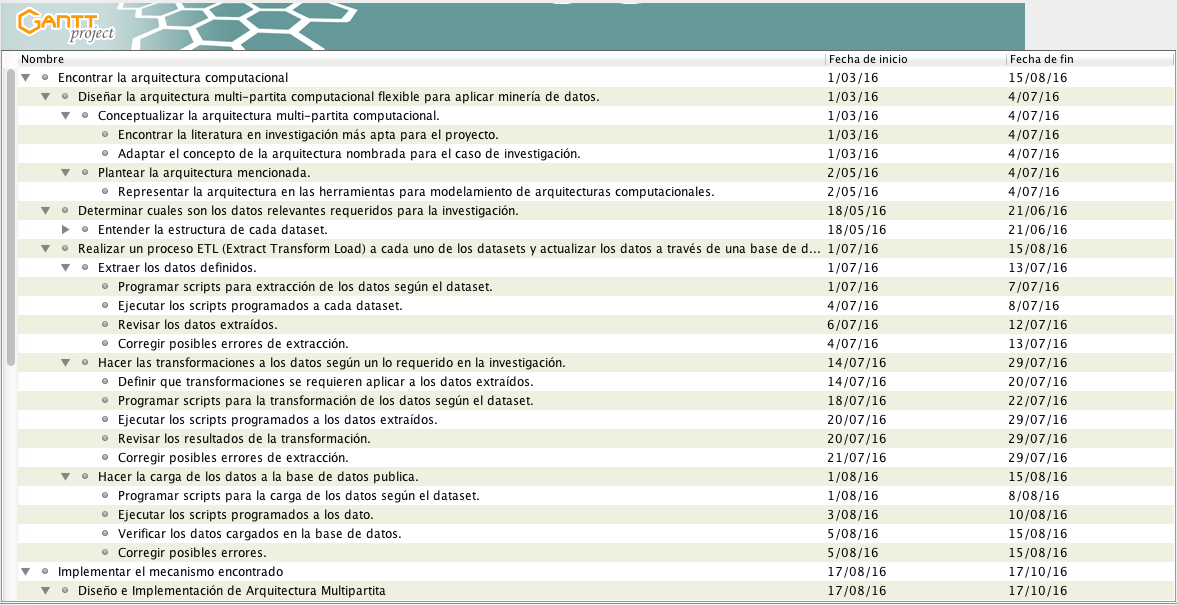
\includegraphics[width=\textwidth]{Imagen1.png}
\end{center}
\end{sidewaystable}
\clearpage

\begin{sidewaystable}
\begin{center}
Parte 2
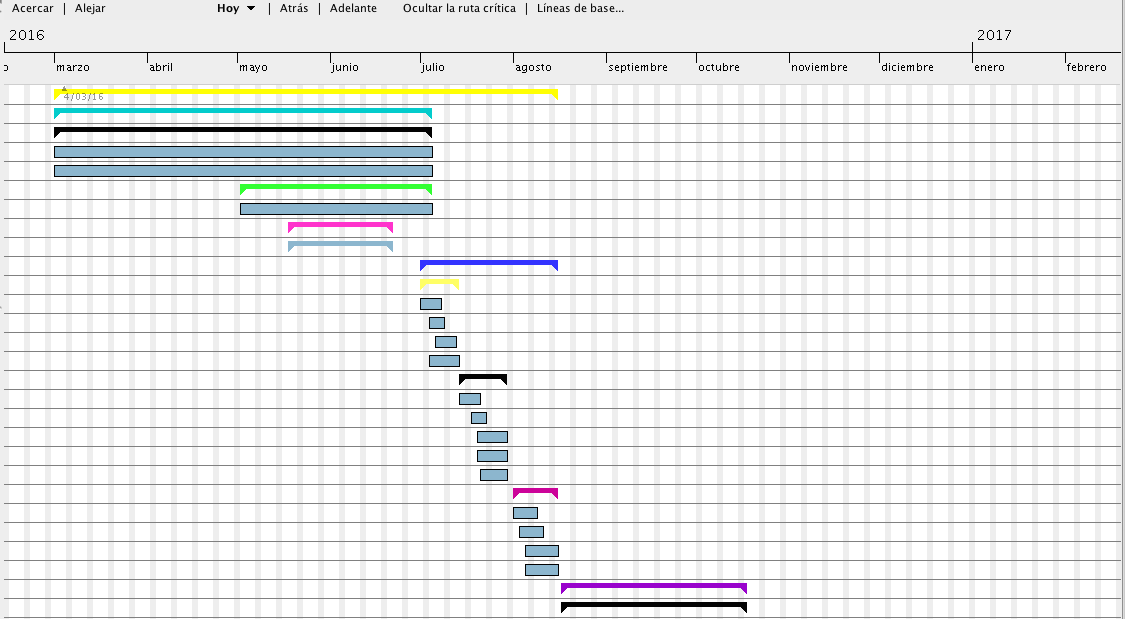
\includegraphics[width=\textwidth]{Imagen3.png}
\end{center}
\end{sidewaystable}
\clearpage

\begin{sidewaystable}
\begin{center}
Parte 3
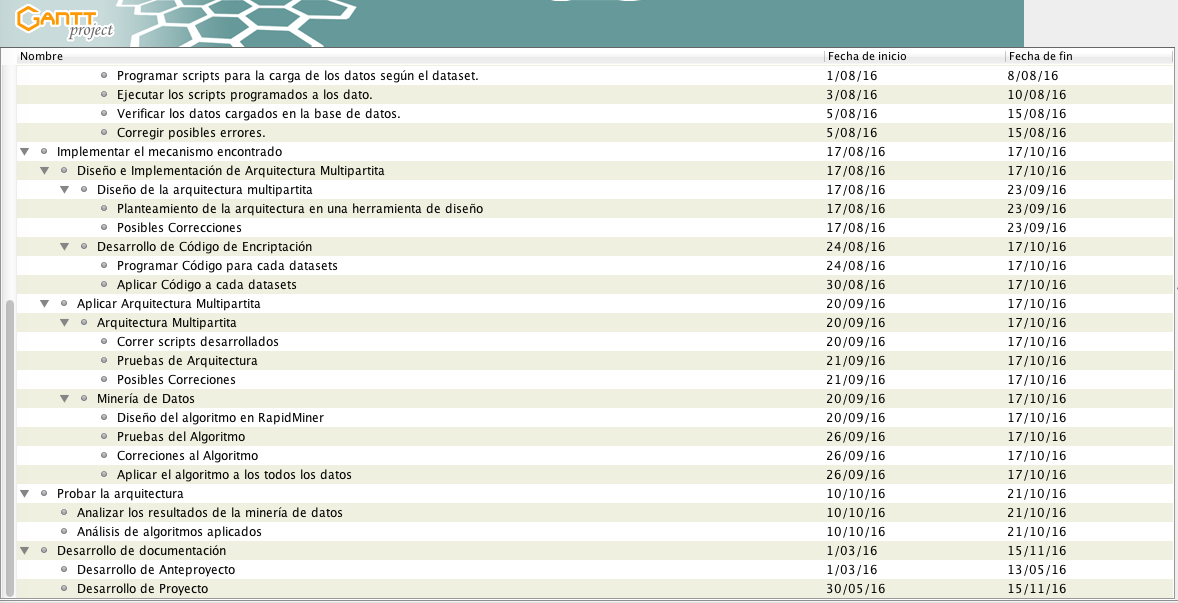
\includegraphics[width=\textwidth]{Imagen2.png}
\end{center}
\end{sidewaystable}
\clearpage

\begin{sidewaystable}
\begin{center}
Parte 4
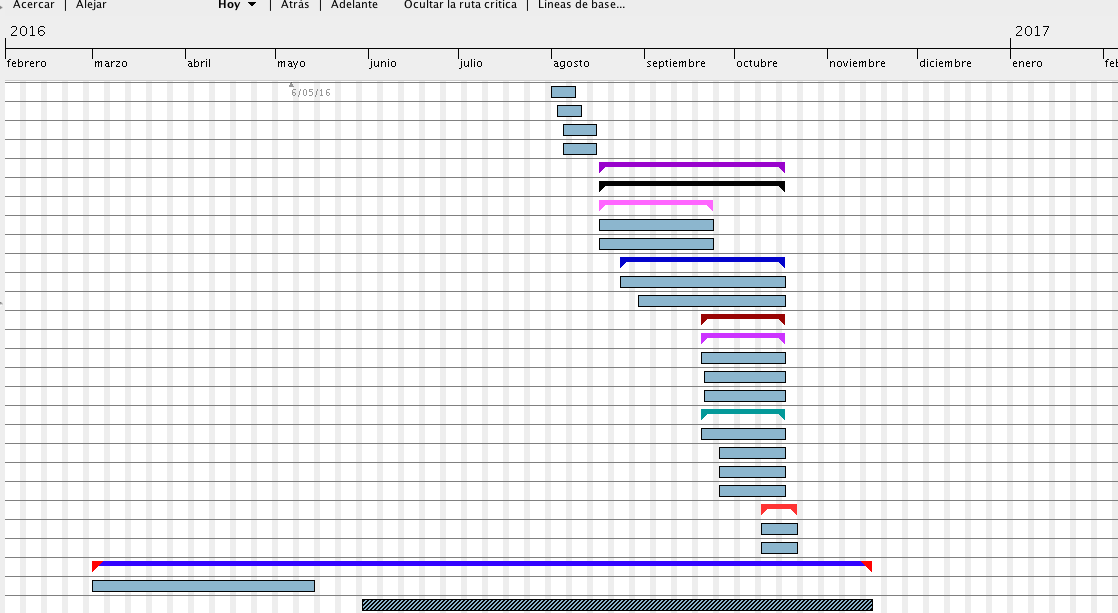
\includegraphics[width=\textwidth]{Imagen4.png}
\end{center}
\end{sidewaystable}
\clearpage

\begin{sidewaystable}
\begin{center}
\section{RECURSOS}
\end{center}
\begin{center}
Parte 1
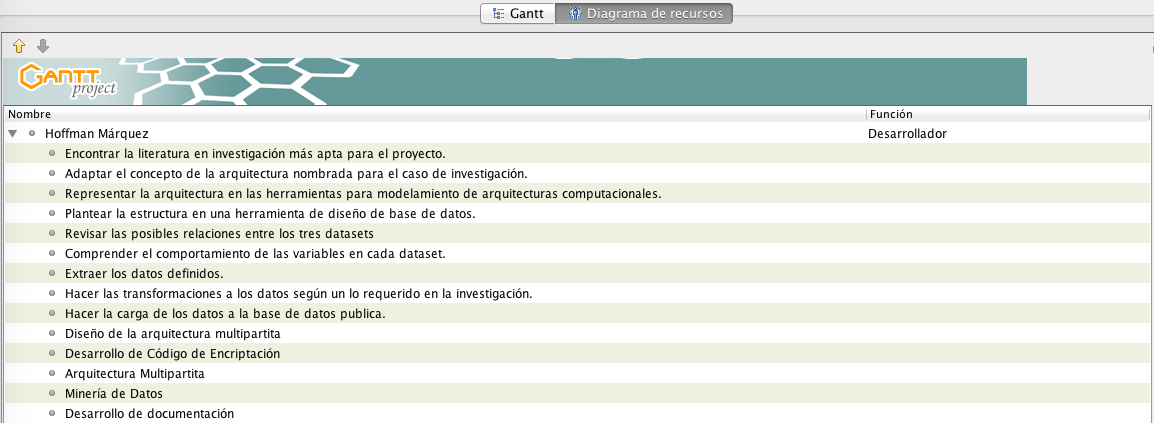
\includegraphics[width=\textwidth]{Hoffman1.png}
\end{center}
\end{sidewaystable}
\clearpage

\begin{sidewaystable}
\begin{center}
Parte 2
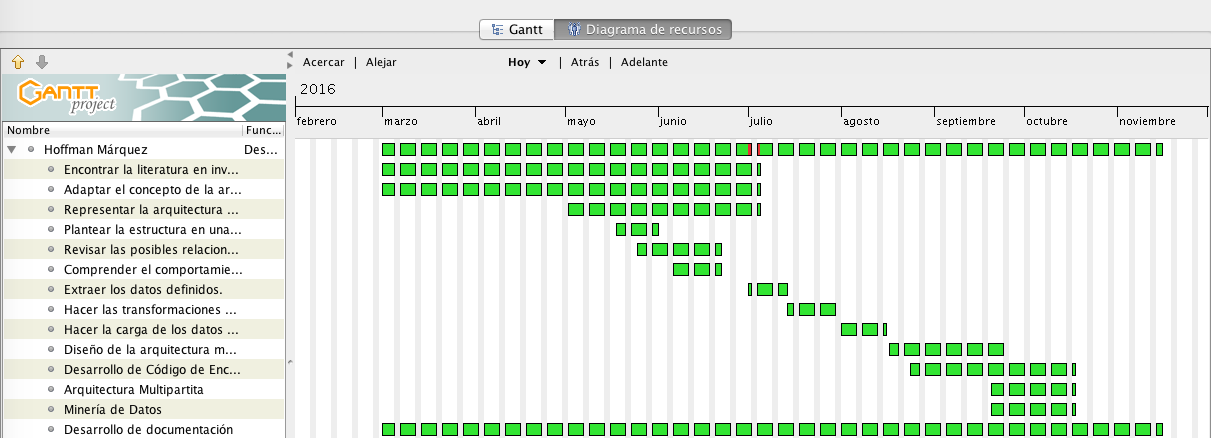
\includegraphics[width=\textwidth]{Hoffma2.png}
\end{center}
\end{sidewaystable}
\clearpage

\begin{sidewaystable}
\begin{center}
Parte 3
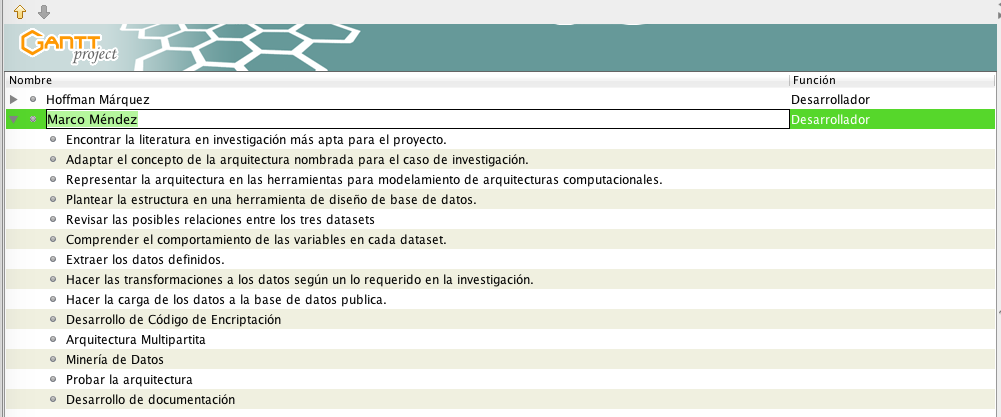
\includegraphics[width=\textwidth]{Marco1.png}
\end{center}
\end{sidewaystable}
\clearpage

\begin{sidewaystable}
\begin{center}
Parte 4
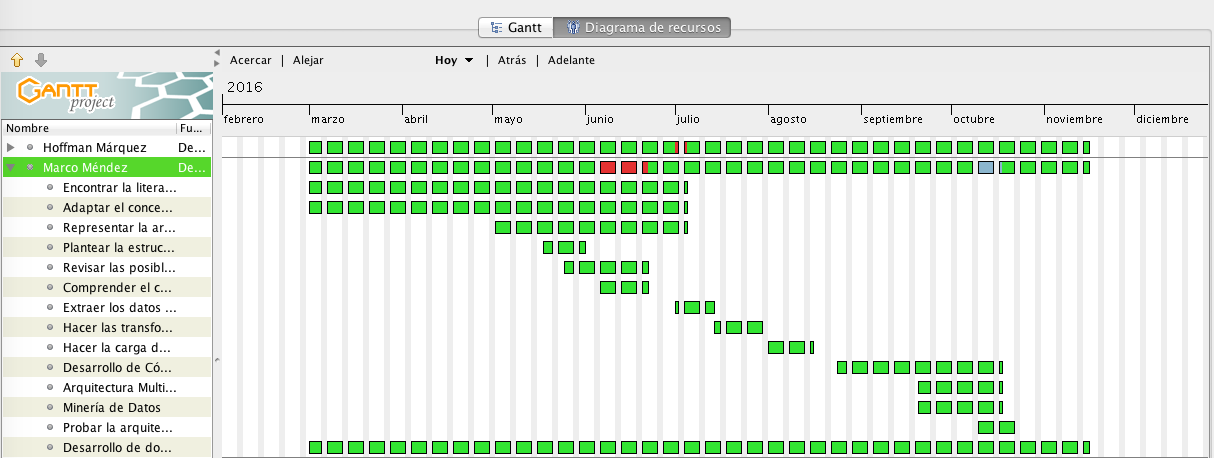
\includegraphics[width=\textwidth]{Marco2.png}
\end{center}
\end{sidewaystable}
\clearpage

\clearpage



% Bibliografa.
%-----------------------------------------------------------------

\begin{thebibliography}{99}


\bibitem[1]{DAN Goodin.}DAN Goodin.\emph{Poorly anonymized logs reveal NYC cab drivers’ detailed whereabouts [En linea]. New York: Dirección URL: <http://arstechnica.com/tech-policy/2014/06/poorly-anonymized-logs-reveal-nyc-cab-drivers-detailed-whereabouts/>. [30, Marzo 2015].}

\bibitem[2]{HERNANDEZ ALEXANDER.}HERNANDEZ ALEXANDER.\emph{New York taxi details can be extracted from anonymised data, researchers say [En linea]. New York: Dirección URL: <https://www.theguardian.com/technology/2014/jun/27/new-york-taxi-details-anonymised-data-researchers-warn>. [30, Marzo 2015].}

\bibitem[3]{HERRANZ Javier NIN Jordi.}HERRANZ Javier , NIN Jordi.\emph{Secure and efficient anonymization of distributed confidential databases, Springer-Verlag Berlin Heidelberg 2014, Online: 23 April 2014. Int. J. Inf. Secur. (2014) 13:497–512, Pág 4.}

\bibitem[4]{DAMGARD Ivan, PASTRO Valerio, SMART Nigel, ZAKARIAS Sarah .}DAMGARD Ivan, PASTRO Valerio, SMART Nigel, ZAKARIAS Sarah .\emph{Multiparty Computation from Somewhat Homomorphic Encryption, International Association for Cryptologic Research 2012, R. Safavi-Naini and R. Canetti (Eds.): CRYPTO 2012, LNCS 7417, pp. 643.}

\bibitem[5]{GHODOSI Hossein Ghodosi, PIEPRZYK Josef, STEINFELD Ron.}GHODOSI Hossein Ghodosi, PIEPRZYK Josef, STEINFELD Ron .\emph{Multi-party computation with conversion of secret sharing, Springer Science+Business Media, LLC 2011, Des. Codes Cryptogr. (2012) 62:259–272, Online: 10 May 2011,pp. 260.}

\bibitem[6]{KIRAZ SABIR Mehmet, UZUNKOL Osmanbey.}KIRAZ SABIR Mehmet, UZUNKOL Osmanbey .\emph{Efficient and verifiable algorithms for secure outsourcing of cryptographic computations, Springer-Verlag Berlin Heidelberg 2015, Int. J. Inf. Secur, Online: 15 Nov 2015,pp. 1.}

\bibitem[7]{LAUD Peeter.}LAUD Peeter .\emph{Privacy-Preserving Minimum Spanning Trees through Oblivious Parallel RAM for Secure Multiparty Computation, Online: 25 Nov 2014,pp. 3.}

\bibitem[8]{LAUD Peeter.}LAUD Peeter .\emph{Privacy-Preserving Minimum Spanning Trees through Oblivious Parallel RAM for Secure Multiparty Computation, Online: 25 Nov 2014,pp. 5.}

\bibitem[9]{GAITAN Mauricio, CANCINO Juliana, BEHRENTZ Eduardo.} GAITAN Mauricio, CANCINO Juliana, BEHRENTZ Eduardo .\emph{Análisis del estado de la calidad del aire en Bogotá, Online: 1 OCT 2007,pp. 3.}

\bibitem[10]{CORREAL Maria Elsa Correal, MARTHA Juan Esteban, SARMIENTO Rodrigo.} GCORREAL María Elsa Correal, MARTHÁ Juan Esteban, SARMIENTO Rodrigo .\emph{Influencia de la variabilidad climática en las enfermedades respiratorias agudas en Bogotá, 2013, Biomédica 2015;35(Supl.2):130-8, <http://dx.doi.org/10.7705/biomedica.v35i0.2456> , pp. 131.}

\bibitem[11]{CORREAL Maria Elsa Correal, MARTHA Juan Esteban, SARMIENTO Rodrigo.} GCORREAL María Elsa Correal, MARTHÁ Juan Esteban, SARMIENTO Rodrigo .\emph{Influencia de la variabilidad climática en las enfermedades respiratorias agudas en Bogotá, 2013, Biomédica 2015;35(Supl.2):130-8, <http://dx.doi.org/10.7705/biomedica.v35i0.2456> , pp. 131.}

\bibitem[12]{CORREAL Maria Elsa Correal, MARTHA Juan Esteban, SARMIENTO Rodrigo.} GCORREAL María Elsa Correal, MARTHÁ Juan Esteban, SARMIENTO Rodrigo .\emph{Influencia de la variabilidad climática en las enfermedades respiratorias agudas en Bogotá, 2013, Biomédica 2015;35(Supl.2):130-8, <http://dx.doi.org/10.7705/biomedica.v35i0.2456> , pp. 133.}

\bibitem[13]{KIRAZ SABIR Mehmet, UZUNKOL Osmanbey.}KIRAZ SABIR Mehmet, UZUNKOL Osmanbey .\emph{Efficient and verifiable algorithms for secure outsourcing of cryptographic computations, Springer-Verlag Berlin Heidelberg 2015, Int. J. Inf. Secur, Online: 15 Nov 2015,pp. 2.}

\bibitem[14]{KIRAZ SABIR Mehmet, UZUNKOL Osmanbey.}KIRAZ SABIR Mehmet, UZUNKOL Osmanbey .\emph{Efficient and verifiable algorithms for secure outsourcing of cryptographic computations, Springer-Verlag Berlin Heidelberg 2015, Int. J. Inf. Secur, Online: 15 Nov 2015,pp. 4.}

\bibitem[15]{GHODOSI Hossein Ghodosi, PIEPRZYK Josef, STEINFELD Ron.}GHODOSI Hossein Ghodosi, PIEPRZYK Josef, STEINFELD Ron .\emph{Multi-party computation with conversion of secret sharing, Springer Science+Business Media, LLC 2011, Des. Codes Cryptogr. (2012) 62:259–272, Online: 10 May 2011,pp. 263.}

\end{thebibliography}
\end{document}